\que{Тензор напряжений Коши, физический  смысл компонент тензора  напряжений Коши. Тензор напряжений Пиолы-Кирхгофа, физический  смысл компонент тензора  напряжений Пиолы-Кирхгофа.}

\paragraph{Тензор напряжений Коши и Пиолы-Кирхгофа.}

Тензор истинных напряжений Коши $\mathbf{T}$ определяется формулами:
\begin{gather*}
	\mathbf{T} = \sum\limits_{\alpha = 1}^{3} \mathbf{r}_{\alpha} \otimes \mathbf{t}^{\alpha} = \mathbf{r}_{i} \otimes \mathbf{t}^i, \\
	\mathbf{t}^{\alpha} \equiv \mathbf{t}_{\alpha} \sqrt{g^{\alpha\alpha}}, \\
	\mathbf{t}_{n} = \mathbf{n} \cdot \mathbf{T}.
\end{gather*}

Как и всякий тензор второго ранга его можно разложить по любому тензорному базису, например:
\begin{equation*}
	\mathbf{T} = T^{ij} \mathbf{r}_i \otimes \mathbf{r}_j = T_{ij} \mathbf{r}^{i} \otimes \mathbf{r}^{j}.
\end{equation*}

\begin{figure}[H]
	\centering
	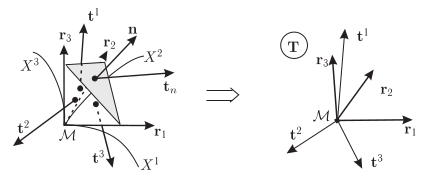
\includegraphics[width=0.6\linewidth]{img/que18}
	\caption{Геометрическое изображение тензора напряжений Коши}
	\label{fig:que18}
\end{figure}

Действительно, если выбрать векторы $\mathbf{r}_i$ в качестве левых векторов, а $\mathbf{t}^i$ рассматривать как правые векторы, то можно перейти к представлению тензора $\mathbf{T}$ в виде классов эквивалентности 
\begin{equation*}
	\mathbf{T} = \mathbf{r}_i \otimes \mathbf{t}^i = \left[\mathbf{r}_1 \mathbf{t}^1 \mathbf{r}_2 \mathbf{t}^2 \mathbf{r}_3 \mathbf{t}^3\right].
\end{equation*}

Тензор напряжений Коши $\mathbf{T}$ определен на площадке $d\Sigma$ в актуальной конфигурации (деформируемой площадке). Можно определить тензор напряжений и на соответствующей $d\mathring{\Sigma}$ в отсчетной конфигурации (недеформированной площадке). Для этого используем соотношение, связывающее $\mathcal{K}$ и $\mathring{\mathcal{K}}$:
\begin{equation*}
	\mathbf{n} d\Sigma = \sqrt{g / \mathring{g}} \, \mathring{\mathbf{n}} \cdot \mathbf{F}^{-1} \, d\mathring{\Sigma}_0,
\end{equation*} 
и рассмотрим вектор напряжений $\mathbf{t}_n$ на площадке $d\Sigma$:
\begin{equation*}
	\mathbf{t}_n \, d\Sigma = \mathbf{n} \cdot \mathbf{T} \, d\Sigma = \sqrt{g / \mathring{g}} \mathring{\mathbf{n}} \cdot \mathbf{F}^{-1} \cdot \mathbf{T} \, d\mathring{\Sigma} = \mathring{\mathbf{n}} \cdot \mathbf{P} \, d\mathring{\Sigma} = \mathring{\mathbf{t}}_n \, d\mathring{\Sigma}.
\end{equation*}

\begin{wrapfigure}[13]{l}{0.5\textwidth}
	\centering
	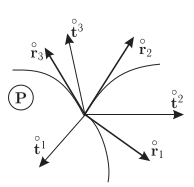
\includegraphics[width=0.45\linewidth]{img/que18_4}
	\caption{Геометрическое изображение тензора напряжений Пиолы-Кирхгофа $\mathbf{P}$}
	\label{fig:que18_4}
\end{wrapfigure}


Здесь введен тензор 
\begin{equation*}
	\mathbf{P} = \sqrt{g / \mathring{g}} \, \mathbf{F}^{-1} \cdot \mathbf{T},
\end{equation*}
называемый \textit{первым тензором напряжений Пиолы-Кирхгофа}, который очевидно определен на недеформированной площадке $d\mathring{\Sigma}$. 

Вектор $\mathring{\mathbf{t}}_n$ называют \textit{вектором напряжений Пиолы-Кирхгофа}, он связан с тензором $\mathbf{P}$ формулой Коши:
\begin{equation*}
	\mathring{\mathbf{t}}_n = \mathring{\mathbf{n}} \cdot \mathbf{P}.
\end{equation*}

Выражение можно представить в виде классов эквивалентности:
\begin{equation*}
	\mathbf{P} = \mathring{\mathbf{r}}_i \otimes \mathring{\mathbf{t}}^i = \left[\mathring{\mathbf{r}}_1 \mathring{\mathbf{t}}^1 \mathring{\mathbf{r}}_2 \mathring{\mathbf{t}}^2 \mathring{\mathbf{r}}_3 \mathring{\mathbf{t}}^3\right], 
\end{equation*}
где обозначены векторы
\begin{equation*}
	\mathring{\mathbf{t}}^{\alpha} = \mathbf{t}_{\alpha} \sqrt{g^{\alpha \alpha} g / \mathring{g}}.
\end{equation*}

С помощью этого представления можно также дать геометрическое изображение тензора Пиолы-Кирхгофа в базисе $\mathring{\mathbf{r}}_i$ отсчетной конфигурации.

\paragraph{Физический смысл компонент тензора Коши.}


\begin{figure}[H]
	\centering
	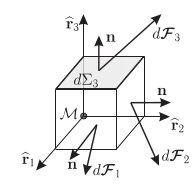
\includegraphics[width=0.4\linewidth]{img/que18_2}
	\caption{К вопросу о физическом смысле компонент тензора напряжений Коши}
	\label{fig:que18_2}
\end{figure}

Пусть в $\mathcal{K}$ имеется локальный базис $\mathbf{r}_i$, мы всегда можем построить ортогональный базис $\widetilde{\mathbf{r}}_i$, а затем, нормируя, ортонормированный $\widehat{\mathbf{r}}_i$, который мы называем \textit{физическим базисом}. В этом базисе тензор напряжений Коши имеет компоненты $\widehat{T}^{ij}$, совпадающие с $\widehat{T}_{ij}$: 
\begin{equation*}
	\mathbf{T} = \widehat{T}^{i j} \widehat{\mathbf{r}}_i \otimes \widehat{\mathbf{r}}_j.
\end{equation*}
Выберем теперь произвольную материальную точку $\mathcal{M} \in V$ и рассмотрим элементарный объем $dV \in V$, содержащий эту точку и имеющий форму куба, грани которого ортогональны векторам $\widehat{\mathbf{r}}_{\alpha}, \, \alpha 1, 2, 3$. Поскольку мы рассматриваем элементарный объем $dV$, то тензор напряжений $\mathbf{T}(x)$ одинаков в каждой точке $\mathbf{x} \in dV$ и $d\Sigma_{\alpha}$, $\alpha = 1, 2, 3$. 

На каждой грани $d\Sigma_{\alpha}$ действует поверхностная сила $d\mathcal{F}_{\alpha}$, связанная с вектором напряжений $\mathbf{t}_{n}$ на этой грани соотношениями плотности внутренних поверхностных сил:
\begin{equation*}
	\text{на } d\Sigma_{\alpha}: \quad \frac{d \mathcal{F}_{\alpha}}{d \Sigma_{\alpha}} = \mathbf{t}_n = \mathbf{n} \cdot \mathbf{T}.
\end{equation*}

Представляя векторы $d\mathcal{F}_{\alpha}$ и $\mathbf{n}$ в базисе $\widehat{\mathbf{r}}_i$:
\begin{equation*}
	d\mathcal{F}_{\alpha} = d\tensor{\mathcal{F}}{^i_{\alpha}} \widehat{\mathbf{r}}_i, \quad \mathbf{n} = \widehat{n}^i \widehat{\mathbf{r}}_i,
\end{equation*}
получаем: 
\begin{equation*}
	\text{на } d\Sigma_{\alpha}: \quad \frac{d\tensor{\mathcal{F}}{^i_{\alpha}}}{d\Sigma_{\alpha}} = \widehat{n}_j \widehat{T}^{ji} = \widehat{T}^{\alpha i}, \quad \alpha = 1, 2, 3,
\end{equation*}
так как на $d\Sigma_{\alpha}: \widehat{n}_{\beta} = \widehat{n}_{\gamma} = 0, \, \alpha \not = \beta \not = \gamma \not = \alpha$. 

Это позволяет прояснить физический смысл компонент $\widehat{T}^{ij}$ тензора напряжений Коши:
\begin{equation*}
	\text{на } d\Sigma_{\alpha}: \quad \widehat{T}^{\alpha\alpha} = \frac{d \mathcal{F}^{\alpha}_{\alpha}}{d\Sigma_{\alpha}}, \, \widehat{T}^{\alpha\beta} = \frac{d\mathcal{F}^{\beta}_{\alpha}}{d\Sigma_{\alpha}}, \, \widehat{T}^{\alpha \gamma} = \frac{d \mathcal{F}^{\gamma}_{\alpha}}{d\Sigma_{\alpha}}, \, \alpha \not = \beta \not = \gamma \not = \alpha.
\end{equation*}

\textit{Нормальные напряжения} $\widehat{T}^{\alpha \alpha}$ --- это отношение соответствующей нормальной компоненты $d\mathcal{F}^{\alpha}_{\alpha}$
 поверхностной силы $d\mathcal{F}_{\alpha}$, действующей на площадке $d\Sigma_{\alpha}$, к величине этой площадки, а \textit{касательные напряжения} $\widehat{T}^{\alpha \beta}, \widehat{T}^{\alpha \gamma}$ --- это отношения касательных компонент $d\mathcal{F}^{\beta}_{\alpha}, d\mathcal{F}^{\gamma}_{\alpha}$ той же силы $d\mathcal{F}_{\alpha}$, действующей на площадке $d\Sigma_{\alpha}$, к величине этой же площадки.

\begin{remark*}
	Поскольку $\mathbf{T}$ одинаков во всем кубе $dV$, то, вследствии первой теоремы Коши, силы $d\mathcal{F}_{\alpha}$ на противоположных гранях куба отличаются только знаком, поэтому соотношения для нормальных и касательных напряжений одни и те же. 
\end{remark*}

\begin{remark*}
	В силу сказанного, различных соотношений --- по три на каждой из трех граней $d\Sigma_{\alpha}$, т.е. всего девять соотношений: для трех нормальных напряжений $\widehat{T}^{\alpha \alpha}$ и шести касательных напряжений $\widehat{T}^{\alpha \beta}, \, \alpha \not = \beta$. 
\end{remark*}

\paragraph{Физический смысл компонент тензора Пиола-Кирхгофа.}

В ортонормированном базисе $\widehat{\mathring{\mathbf{r}}}_i$ отсчетной конфигурации:
\begin{equation*}
	\mathbf{P} = \widehat{P}^{ij} \widehat{\mathring{\mathbf{r}}}_i \otimes \widehat{\mathring{\mathbf{r}}}_j.
\end{equation*}

Выберем в $\mathring{\mathcal{K}}$ материальную точку $\mathcal{M}$ и рассмотрим элементарный объем $d\mathring{V}$ в форме куба, содержащий эту точку. Грани куба $d\mathring{\Sigma}_{\alpha}$, как и ранее, выберем ортогональными векторам $\widehat{\mathring{\mathbf{r}}}_{\alpha}$.

Этому кубу $d\mathring{V}$ в конфигурации $\mathcal{K}$ соответствует искаженный объем $dV$. В силу геометрической картины преобразования материальной точки сплошной среды, объем $dV$ будет иметь форму параллелепипеда, вообще говоря, с наклонными гранями $d\Sigma_{\alpha}$, но остающимися плоскими.

\begin{figure}[H]
	\centering
	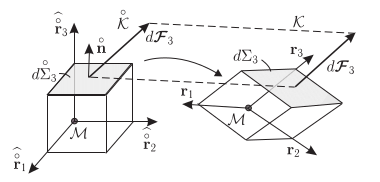
\includegraphics[width=0.6\linewidth]{img/que18_3}
	\caption{К вопросу о физическом смысле компонент тензора напряжений Пиолы-Кирхгофа}
	\label{fig:que18_3}
\end{figure}

 Для элементарных объемов $d\mathring{V}$ и $dV$ тензоры напряжений $\mathbf{T}(\mathbf{x})$ и $\mathbf{P}(\mathring{\mathbf{x}})$ одинаковы в каждой точке $\mathbf{x} \in \overline{dV}$ и $\mathring{\mathbf{x}} \in \mathring{\overline{dV}}$. 
 
 На деформированной (но плоской) грани $d\Sigma_{\alpha}$ действует поверхностная сила $d\mathcal{F}_{\alpha}$. Перенесем ее параллельным переносом в $\mathring{\mathcal{K}}$ на соответствующую грань $d\mathring{\Sigma}_{\alpha}$, тогда на грани $d\mathring{\Sigma}_{\alpha}$ можно записать следующие соотношения:
 \begin{equation*}
 	\text{на } d\mathring{\Sigma}_{\alpha} : \quad \frac{d\mathcal{F}_{\alpha}}{d\Sigma_{\alpha}} \left(\frac{d\Sigma_{\alpha}}{d\mathring{\Sigma}_{\alpha}}\right) = \mathbf{t}_n \left(\frac{d\Sigma_{\alpha}}{d\mathring{\Sigma}_{\alpha}}\right) = \mathring{\mathbf{n}} \cdot \mathbf{P}.
 \end{equation*}
 
 Представляя векторы $d\mathcal{F}_{\alpha}$ и $\mathring{\mathbf{n}}$ в базисе $\widehat{\mathring{\mathbf{r}}}_i$: 
 \begin{equation*}
 	d\mathcal{F}_{\alpha} = d\tensor{\mathring{\mathcal{F}}}{^i_{\alpha}} \widehat{\mathring{\mathbf{r}}}_i, \quad \mathring{\mathbf{n}} = \widehat{\mathring{n}}^i \widehat{\mathring{\mathbf{r}}}_i,
 \end{equation*}
 и из соотношений на $d\mathring{\Sigma}_{\alpha}$ получаем:
 \begin{equation*}
 	\text{на } d\mathring{\Sigma}_{\alpha} : \quad \frac{d\tensor{\mathring{\mathcal{F}}}{^i_{\alpha}}}{d\Sigma_{\alpha}} = \widehat{\mathring{n}} \widehat{P}^{ij} = \widehat{P}^{\alpha i}, \quad \alpha = 1, 2, 3, 
 \end{equation*}
 т.к. на $\mathring{\Sigma}_{\alpha} : \widehat{\mathring{n}}_\alpha = 1$, а $\widehat{\mathring{n}}_{\beta} = \widehat{\mathring{n}}_{\gamma} = 0$. 

Итого, получаем:
\begin{equation*}
	\text{на } d\mathring{\Sigma}_{\alpha} : \quad \widehat{P}^{\alpha\alpha} = \frac{d\mathring{\mathcal{F}}^{alpha}_{\alpha}}{d\mathring{\Sigma}_{\alpha}}, \quad \widehat{P}^{\alpha \beta} = \frac{d \mathring{\mathcal{F}}^{\beta}_{\alpha}}{d\mathring{\Sigma}_{\alpha}}, \quad \widehat{P}^{\alpha \gamma} = \frac{d \mathring{\mathcal{F}}^{\gamma}_{\alpha}}{d\mathring{\Sigma}_{\alpha}}, \quad \alpha \not = \beta \not = \gamma \not = \alpha.
\end{equation*}

Таким образом, \textit{нормальное напряжение} $\widehat{P}^{\alpha \alpha}$ --- это отношение нормальной компоненты $d\mathring{\mathcal{F}}^{\alpha}_{\alpha}$ поверхностной силы $d\mathcal{F}_{\alpha}$, действующей на деформированной площадке $d\Sigma_{\alpha}$, к величине соответствующей недеформированной площадке $d\mathring{\Sigma}_{\alpha}$. \textit{Касательные напряжения} $\widehat{P}^{\alpha\beta}, \widehat{P}^{\alpha\gamma}$ --- это отношения касательных компонент $d\mathring{\mathcal{F}}^{\beta}_{\alpha}, d\mathring{\mathcal{F}}^{\gamma}_{\alpha}$ той же поверхностной силы $d\mathcal{F}_{\alpha}$, действубщей на деформированной площадке $d\Sigma_{\alpha}$, к величине недеформированной площадки $d\mathring{\Sigma}_{\alpha}$.

Замечания для $\mathbf{T}$ остаются справедливыми и для $\mathbf{P}$. За исключением того, что тензор $\mathbf{P}$ остается несимметричным, даже если $\mathbf{T}$ --- симметричен. 